\documentclass[12pt]{article}
\usepackage{minted}
\usepackage{graphicx}
\usepackage[margin=0.25in]{geometry}

\begin{document} 
	\noindent
	Dan Jandel C. De Ramos\\
	BSCpE 2-1\\
	Made with \LaTeX \\
	GitHub repo link: https://github.com/Joatmon-21/De-Ramos-CMPE201\\
	\\
	Activity 1 (Same as Sample)\\
	Source Code:
	\begin{minted}[tabsize=5]{java}         
/*
* Written by: Dan Jandel C. De Ramos
* Polytechnic University of the Philippines Biñan
* Bachelor of Science in Computer Engineering 2-1
*/
		
public class Activity_1_SAS{
	public static void main(String[]args){         
				
		//The data stored here are for the sake of examples only and are not 100% accurate        
		String name = "Juan S. Dela Cruz";        
		char gender = 'm';        
		boolean maritalStatus = true;
		byte numberOfChildren = 8;
		short birthYear = 1945;
		int salary = 88000;  
		long netAsset = 8234567890L;
		double weight = 88.88;
		float gpa = 3.88f;
				
		System.out.println("Name is : " + name);
		System.out.println("Gender is : " + gender);
		System.out.println("Is married is : " + maritalStatus);
		System.out.println("Number of Children is : " + numberOfChildren);
		System.out.println("Year of birth is : " + birthYear);
		System.out.println("Salary is : " + salary);
		System.out.println("Net Asset is : " + netAsset);
		System.out.println("Weight is : " + weight);
		System.out.println("GPA is : " + gpa);       
	}
}
	\end{minted}
	\clearpage
	\noindent
	Output:\\
	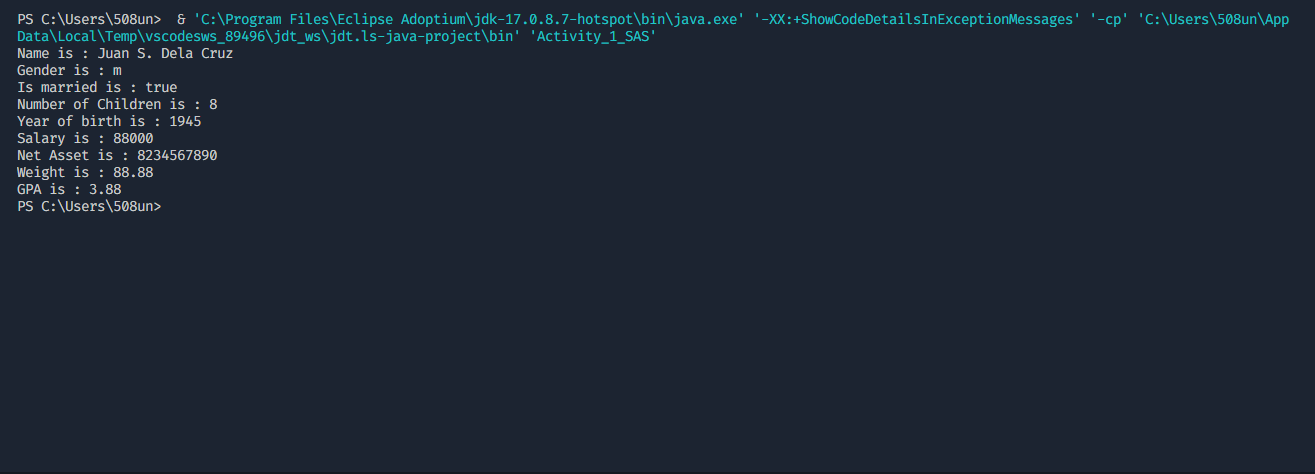
\includegraphics[width=\textwidth]{output1SAS}
\end{document}